% ------ headers globales y begin ---------------
\documentclass[11pt, a4paper, twoside]{article}
\usepackage{header_tp1}

\begin{document}{}
% -----------------------------------------------

\subsubsection{Descripción} \label{subsubsec:problema1-descripcion}
%-
%- PLANTEO DEL PROBLEMA
%-
\centerbf{Planteo del problema}

El inspector \texttt{Rick A. Lapazta}, legendario\footnote{La leyenda dice que
junto a su compañero Zepas A. Poraki, son invictos en no hacer muy bien su
trabajo} empleado un puesto de control de camiones, es encomendado por la diosa
Mor\texttt{fea} durante un revelador sueño a la tarea de investigar si la
empresa \textit{il Ravioli} está transportando \texttt{sustancias ilegales}.
Luego de meses de investigación, y de arriesgar su pasiva e inspeccionista vida
intrusionando en el archivo secreto de la empresa descubre que realmente cuenta
con muy poca información: dispone de una lista en la anotó los datos importantes
de cada camión, la cantidad de antenas de cada uno de ellos, y el día en que
atravesarán el control. El inspector deduce posteriormente que la mayor o menor
cantidad de antenas de un camión no debe ser un factor influyente al momento de
transportar este tipo de sustancias, y que la mejor solución a sus problemas es
contratar a un \textit{experto}.

Como dispone de una cantidad acotada de dinero, y sabe que el tercerizado le
cobrará una cantidad fija de dinero por cada día de trabajo el inspector busca,
dado un rango de días de inspección, maximizar la cantidad de camiones
inspeccionados, es decir que la mayor cantidad de camiones tienen que estar
pasando por el puesto durante el período de contración del experto. El inspector
conoce los días en que cada uno de los $n$ camiones de la empresa estará
pasando, pero desgraciadamente esta información puede o no estar dada en orden
cronológico, nadie lo sabe. El inspector olvidó mencionarlo, pero el experto es
de otro país, el reino de muy muy lejano, y la legislación de turismo de la zona
es muy dura, por lo que este sólo dispone de permiso realizar un viaje al puesto
de inspección.

%-
%- FORMATO DE LOS DATOS
%-
\centerbf{Formato de los datos}

El problema encomienda encontrar una solución al dilema del inspector, en donde
recibiendo como \textbf{datos de entrada} la cantidad de días ($D$), la cantidad
de camiones ($n$) y los días en que estos llegarán ($d_1$,$d_2$,...,$d_n$) se
deberá idear un algoritmo que lo resuelva con una complejidad
\textbf{estrictamente mejor que} \bigO{n^{2}}, siendo $n$ la cantidad total de
camiones. El resultado que se deberá obtener es el día inicial $d_i$ en que
convendría contratar al experto, y el total $c$ de camiones que serán
inspeccionados por el mismo.

% primera columna
\begin{minipage}[t]{0.5\textwidth}
\centerbf{Formato de entrada}
\[
  D\ n\ d_{1}\ d_{2}\ ...\ d_{n}\
\]

\end{minipage}
% segunda columna
\begin{minipage}[t]{0.5\textwidth}
\centerbf{Formato de salida}
\[
  d_{i}\ c
\]

\end{minipage}

%-
%- INTERPRETACION DEL PROBLEMA
%-
\newpage
\centerbf{Interpretación del problema (ejemplos)}

\begin{ejemplo}\hspace{0em}

Si se contratase al experto por $D=3$ días consecutivos y en total hubiesen $n=20$
camiones sospechosos ($c1,c2,...,c20$), se podría tener una entrada como la siguiente:

  \begin{quote}
    \begin{verbatim}
    Entrada:
    3 20 10 10 9 4 1 1 1 1 1 2 6 6 6 4 5 5 5 5 5 9
    \end{verbatim}
  \end{quote}
  
  \vspace{-2em}
    \begin{center}
      La cual se podría visualizar de la siguiente forma:
      
      \renewcommand{\arraystretch}{1.2} % Agrego un poco de margen vertical
      \begin{tabular}{|c|c|c|c|c|c|c|c|c|c|c|}
        \hline
        Día          &  $1$  & $2$   & $3$   & $4$   & $5$   & $6$ & $7$ & $8$ & $9$   & $10$  \\
        \hline
                     & $c5$ & $c10$ & $c14$ & $c4$ & $c15$ & $c11$ &   &     & $c3$  & $c1$  \\
                     & $c6$ &       &       &       & $c16$ & $c12$ &   &     & $c20$ & $c2$  \\    
        Camiones     & $c7$ &       &       &       & $c17$ & $c13$ &   &     &       &       \\  
                     & $c8$ &       &       &       & $c18$ &       &   &     &       &       \\
                     & $c9$ &       &       &       & $c19$ &       &   &     &       &       \\
        \hline
      \end{tabular}
    \end{center}

    En este caso, como el primer día del período de contratación sería $d=4$ y habrían sido
    inspeccionados un total de $C=9$ camiones durante los días \texttt{Día4}, \texttt{Día5} 
    y \texttt{Día6} el programa debería devolver la siguiente salida: 

  \begin{quote}
    \begin{verbatim}
    Salida:
    4 9
    \end{verbatim}
  \end{quote}

\end{ejemplo}

\begin{ejemplo}\hspace{0em}

Bajo las mismas condiciones del ejemplo anterior, también 
se podría tener una entrada como la siguiente:

  \begin{quote}
    \begin{verbatim}
    Entrada:
    3 20 1 2 7 1 1 1 1 1 1 1 7 7 7 1 4 4 4 4 4 7
    \end{verbatim}
  \end{quote}

  \vspace{-2em}
  \begin{center}
    La cual se podría visualizar de la siguiente forma:
    
    \renewcommand{\arraystretch}{1.2} % Agrego un poco de margen vertical
    \begin{tabular}{|c|c|c|c|c|c|c|c|}
      \hline
      Día          &  $1$  & $2$   & $3$   & $4$    & $5$ & $6$ & $7$   \\
      \hline
                     &  $c5$ &       &       & $c15$  &     &     & $c11$ \\
                     &  $c6$ &       &       & $c16$  &     &     & $c12$ \\    
                     &  $c7$ &       &       & $c17$  &     &     & $c13$ \\  
                     &  $c8$ &       &       & $c18$  &     &     & $c3$  \\
      Camiones     &  $c9$ &       &       & $c19$  &     &     & $c20$ \\
                     &  $c10$&       &       &        &     &     &       \\
                     &  $c14$&       &       &        &     &     &       \\
                     &  $c4$ &       &       &        &     &     &       \\
                     &  $c1$ &       &       &        &     &     &       \\
                     &  $c2$ &       &       &        &     &     &       \\
      \hline
    \end{tabular}
  \end{center}

  En este otro caso, el primer día del período de contratación sería $d=1$, en el cual
  habrían sido inspeccionados, durante los días \texttt{Día1}, \texttt{Día2} y
  \texttt{Día3}, un total de $c=10$ camiones:

  \begin{quote}
    \begin{verbatim}
    Salida:
    1 10
    \end{verbatim}
  \end{quote}

\end{ejemplo}

\subsubsection{Planteamiento de resolución}\label{subsubsec:problema1-resolucion}

\centerbf{Caracterización de la solución}

\begin{notacion}
Sean: 
  \begin{itemize}
    \item $D \in \nat$ la cantidad de días que trabaja el inspector
    \item $n \in \nat$ la cantidad total de camiones.
    \item $t \in \nat$ la diferencia entre el último día y el primer día en que pasan camiones.
    \item $c_{i} \in \nat$ el día en que pasará el ``camión i''. \textbf{Notar aquí la diferencia de notación con la notación de entrada}.
  \item $d_{i} \in \Z$ el ``día $i$'', dado por el intervalo determinado por $d_{1} =$ el primer día que pasa un camión, y $d_{t} =$ el último día que pasa un camión. Aclaración: $d_{i}$ puede ser negativo.
  \end{itemize}
\end{notacion}

\begin{proposicion}
Representamos el conjunto \textbf{universo de soluciones} bajo la forma de 
\textbf{$S \subseteq \nat$} en donde, para cada solución, \textbf{$s \in S$} 
representa al día en que se contrata al inspector.
Esta representación es suficiente para generar todo el universo de soluciones únicas.
\end{proposicion}
\begin{demostracion}\label{dem:ej1_1}
\textbf{Bajo las condiciones de una determinada entrada}, asumir que este 
parámetro \textbf{$s$} basta para definir una \textbf{solución única}
es equivalente a decir que
\textbf{existe una función sobreyectiva $\#camiones{:}~S\rightarrow\nat_{0}$}
que, dado un determinado día \textbf{$s$}, devuelve la cantidad de camiones 
inspeccionados para esa solución.

Esto es así porque el inspector trabajará una \textbf{cantidad fija y predeterminda
de días consecutivos} que depende exclusivamente de susodicha entrada, y 
además la cantidad total de camiones inspeccionados es la sumatoria de la cantidad
de camiones inspeccionados en cada uno de los días en que el inspector trabaje.
\end{demostracion}

\begin{definicion}\textbf{Función Objetivo}\label{def:ej1-funcionobjetivo}

Nos interesa elegir cuál es el mejor día entre $d_1$ y $d_{t+1-D}$.Siendo 
camionesEnElDia una función que dado un día devuelve el conjunto de
camiones que circulan en el mismo, buscamos maximizar la siguiente 
\textbf{función objetivo}\ $f:~S~\rightarrow~\nat$:
\[
  \red{f(s)} = \sum_{i=k}^{k+D-1}{|~camionesEnElDia(d_{i})~|}
\]
la cual, además, resulta ser la función mencionada $\#camiones$ mencionada
en \ref{dem:ej1_1}.
\end{definicion}

\begin{proposicion}
Reducimos el intervalo de análisis al rango \textbf{$[d_{1},~d_{t+1-D}] \subset S$},
ya que el resto de las soluciones resultan indiferentes a los objetivos del problema.
\end{proposicion}
\begin{demostracion}
Ya que nos interesa obtener la solución que maximice la cantidad de camiones
inspeccionados (función \ref{def:ej1-funcionobjetivo}), y por el mismo motivo expuesto en la demostración anterior, 
podemos acotar el análisis del universo de soluciones al rango 
\textbf{$[d_{1+1-D},~d_{t}]$} debido a que, ya que \textbf{$d_{1}$} es el día en que 
pasa el primer camión, y \textbf{$d_{t}$} es el día en que pasa el último camión, 
podemos asegurar que para cualquier solución \textbf{s} fuera de este rango
\textbf{$\#camiones(s)~=~0$}. 

Más aún, podemos acotar el análisis al intervalo \textbf{$[d_{1},~d_{t+1-D}]$},
contenido en el intervalo anterior ya que, por las razones antes expuestas, 
podemos asegurar que: 
  
    $\#camiones$ valuada en {$[d_{1+(1-D)},~d_{1})$} es menor o igual
    a $\#camiones(d_{1})$
    
    $\#camiones$ valuada en {$(d_{t+(1-D)},~d_{t}]$} es menor o igual
    a $\#camiones(d_{t+1-D})$.
\end{demostracion}


\begin{proposicion}
Dado un intervalo de análisis, nos interesará inspeccionar sólamente los días
en que haya transcurrido al menos un camión.
\end{proposicion}
\begin{demostracion}
Dado que buscamos maximizar la función objetivo (\ref{def:ej1-funcionobjetivo})
entonces, abreviando camionesEnElDia como cEED,

\begin{eqnarray}
\red{f(s)} &=& \sum_{i=s}^{s+D-1}{|cEED(d_{i})|} \nonumber\\
     &=& |cEED(s)| + \sum_{i=s+1}^{s+D-1}{|cEED(d_{i})|} \nonumber\\
     &=& |cEED(s)| + \sum_{i=s+1}^{s+D-1}{|cEED(d_{i})|} + |cEED(s+D-1+1)| - |cEED(s+D-1+1)| \nonumber\\
     &=& |cEED(s)| + \sum_{i=s+1}^{s+D-1+1}{|cEED(d_{i})|} - |cEED(s+D-1+1)| \nonumber\\
     &=& |cEED(s)| + \red{f(s+1)} - |cEED(s+D-1+1)| \nonumber
\end{eqnarray}

Pero si $|~cEED(s)=0~|$, y dado que cEED es no negativa, entonces se deduce que
\begin{eqnarray}
\red{f(s)} &=& |cEED(s)| + f(s+1) - |cEED(s+D-1+1)| \nonumber \\
     &=& 0 + \red{f(s+1)} - |cEED(s+D-1+1)| \leq \red{f(s+1)} \nonumber
\end{eqnarray}
de lo cual se desprende que 
\[
  s=0 \then f(s) \leq f(s+1)
\]
y como buscamos maximizar f, podemos obviar las soluciones en que s=0.
\end{demostracion}



\centerbf{Pseudocódigo}

Primero, entonces, ordenamos en forma creciente el conjunto
{$c_1$,...,$c_n$}. Sabemos que la solución pertenece a este conjunto.
Según (\ref{def:ej1-funcionobjetivo}), tenemos a \red{$f(s)$} como la sumatoria 
de la cantidad de camiones que pasan desde el día $s$ hasta el día $s+D-1$. 
Nuestro algoritmo itera sobre cada elemento $c_i$ del conjunto, calculando 
para cada uno \red{$f(c_i)$}, y guardando en todo momento el elemento $e$ tal que 
\red{$f(e)$} es el máximo. Al final de las iteraciones, tenemos guardado el
elemento $e$ tal que \red{$f(e)$} es máximo en todo el conjunto de soluciones. 
Devolvemos $e$ y \red{$f(e)$}.


\subsubsection{Justificación formal de correctitud}

Consideremos los días de llegada ordenados en forma creciente: $d_1 \le d_2 \le
\dots \le d_n$ son enteros \underline{positivos} al igual que $D$. \\ Definimos
P(x), donde $x \in \mathbb{N}$, como $\sum_{i=1}^{n} I(d_i)_{[x,x+D-1]}$. \\
Buscamos $d$ tal que $(\forall x)$ P(x) $\le$ P(d). \\ Veamos que $d \le d_n$:
\\ P$(d_n)=1$ pues $d_n \in [d_n,d_n + D - 1]$ pero $\forall x > d_n$, P(x)$=0$
pues $d_i < x, \forall i \in 1...n$.\\ Luego, si $d > d_n, d$ no es óptimo. \\
Veamos que existe un $d$ óptimo tal que $d=d_i$ para algún $i \in 1...n$. \\ Sea
$d'$ óptimo. \\ Sea $d=min_{i \in 1...n}$ $d_i \big| d_i \ge d'$. \\ P(d)$\ge$
P(d') pues $\forall i$ tal que $d_i \in [d',d'+D-1], d_i \in [d,d+D-1]$ ya que
$\nexists$ $j$ tal que $d' \le d_j < d$ y pues $d'+D-1 \le d+D-1$. \\ Luego,
hemos reducido el espacio de solución a $\{$ $d_1,...,d_n$$\}$.


\subsubsection{Cota de complejidad temporal}\label{sec:ej1cotatemporal}
El algoritmo utilizado es el siguiente:

\begin{algorithm}[H]
\caption{Algoritmo Camiones Sospechosos}\label{camionessospechosos}
\footnotesize\begin{algorithmic}[1]
  \Require
    \Statex $intervaloInspector \gets$ \Call{dameIntervaloInspector}{} \Comment{$integer$}
    \Statex $cantidadDeCamiones \gets$ \Call{dameCantidadCamiones}{} \Comment{$integer$}
    \Statex $fechasCamiones \gets$ \Call{dameFechasCamiones}{} \Comment{$arreglo\langle integer \rangle$}
  \Ensure
    \Statex \Call{Fecha Óptima Inspector}{} \Comment{$integer$}
    \Statex \Call{Cantidad De Camiones Analizados}{} \Comment{$integer$}
  \Statex
  
  \State \Call{ordenar}{fechasCamiones} \Comment{\bigO{n.\log n}}
  \State $inicioInter \gets 0$ \Comment{\bigO{1}}
  \State $finInter \gets 0$ \Comment{\bigO{1}}
  \State $mDia \gets 0$ \Comment{\bigO{1}}
  \State $mCantidadCamiones \gets 0$ \Comment{\bigO{1}}

  \While {$finInter < cantidadDeCamiones$} \Comment{ \texttt{Como máximo n interaciones}}
    \While {$ \Call{DiferenciaMenorAInterInspector}{inicioInter, finInter} $}
      \State $ finInter \gets finInter+1$
    \EndWhile 
  \If {$\Call{CantCamionesEn}{inicioInter, finInterl} < mCantidadCamiones$} \Comment{\bigO{1}}
    \State $ mDia \gets inicioInter$ \Comment{\bigO{1}}
    \State $ mCantidadCamiones \gets \Call{CantCamionesEn}{inicioInter,finInter}$ \Comment{\bigO{1}}
  \EndIf {}
  \State $inicioInter \gets inicioInter +1$
  \EndWhile \Comment{\texttt{ciclo} \bigO{n}}
  \State \Return {$mDia, mCantCamiones$}
  \State


  \Function{CantCamionesEn}{$inicioInter, finInter$}
  \State \Return { $finInter - inicioInter$ } \Comment{\bigO{1}}
  \EndFunction \Comment{\texttt{final} \bigO{1}}
  \State

  \Function{DiferenciaMenorAInterInspector}{$inicioInter, finInter$}
    \State $diferencia \gets fechasCamiones_{finInter} - fechasCamiones_{inicioInter}$ \Comment{\bigO{1}}
    \State \Return {$ finInter < cantidadDeCamiones \texttt{ and } diferencia < intervaloInspector $} \Comment{\bigO{1}}
  \EndFunction \Comment{\texttt{final} \bigO{1}}

  \Statex{}
\end{algorithmic}
\end{algorithm}


Consideremos la complejidad del ciclo for. A lo largo del ciclo se van
actualizando izq y der, y se va guardando el maximo que lleva  en si O(1).
¿Cuántas veces se actualizan izq y der? Pues, como van en forma creciente de 1 a
n, exactamente n veces cada una. El ciclo for tiene complejidad O(2n) = O(n). La
complejidad del algoritmo es finalmente O(n log n).

Como se puede ver el algorítmo tiene 2 partes bien diferenciadas: Primero tiene
un ordenamiento de un arreglo unidimensional. Para eso se usa el algorítmo de
ordenamiento que brinda a librería standard de \textit{c++}. En la documentación
de la misma se puede apreciar que su complejidad en el peor caso es de \bigO{n.
\log n}\footnote{http://www.cplusplus.com/reference/algorithm/sort/} donde
\textit{n} es la distancia que hay entre el primer y el último elemento que se
quieren ordenar. En este caso se necesita ordenar todo el arreglo, por lo que
termina siendo \bigO{n.\log n} con respecto al tamaño de la entrada.

Luego hay un bucle while. El bucle \texttt{mientras} se repite mientras que el
fin del intervalo a analizar se encuentre dentro del arreglo de camiones.

Apenas se entra al ciclo \texttt{mientras} hay otro ciclo, el cuál tiene una
complejidad de peor caso de \bigO{n}. Este ciclo interno se encarga de hacer
avanzar el puntero \textit{finInter} hasta que la diferencia entre de las fechas
entre el principio del intervalo a analizar y el final del intervalo a analizar
sea menor a \textit{intervaloInspector}. El peor caso posible en este ciclo
sería que la diferencia entre el la fecha mas próxima y la fecha mas lejana sea
menor a intervalo inspector. En ese caso sale del bucle porque se pasó del
máximo. Sim embargo si eso ocurre también se deja de cumplir la condición de la
guarda externa, por lo tanto el bucle externo también termina.


Es decir, ambas guardas dependen de la misma comparación entre \textit{finInter}
y \textit{cantCamiones}, por lo tanto cuando termine una va a terminar la otra.
Por otra parte \textit{finInter} siempre avanza. No hay ningún caso en el cuál
retroceda. Esto significa que siempre va a recorrer exactamente
\textit{cantCamiones}, es decir que en el peor de los casos va a haber
\texttt{n} iteraciones del ciclo. Como el resto de las operaciones son todas
\bigO{1} podemos concluir que el ciclo completo tiene una complejidad de
\bigO{n}


De esta manera el algorítmo termina teniendo una complejidad de \bigO{n.\log n +
n} = \bigO{n. \log n}. De esta manera la complejidad es estrictamente menor que
$\bigO{n^{2}}$.



\subsubsection{Verificación mediante casos de prueba}

A continuación presentamos distintas instancias que sirven para verificar que el programa funciona correctamente. \\ 
\\
Input: [D n $d_1$...$d_n$], Output: [d c] \\
\\
D: cant. de días de contratación del experto \\
n: cant.  total de camiones que pasan por el puesto \\
$d_i$ con $1 \le i \le n$: días de llegada de los camiones \\
d: día inicial del período de contratación del experto \\
c: cant. de camiones inspeccionados por el experto \\  
\\
Sea $L$ el intervalo de días en que llegan los camiones. \\
$L$ $=$ (máx $d_i$ $-$ mín $d_i$ $+ 1$) con $1 \le i \le n$. \\

De los datos de entrada y salida sabemos que: 

\begin{itemize}
    \item $1$ $\le$ D, n, $d_i$ (con $1$ $\le$ i $\le$ n).
  \item $1 \le $ c $\le$ n 
  \item $1 \le $ mín $d_i$ $\le$ d $\le$ máx $d_i$ 
\end{itemize}

Entonces, podemos separar el conjunto de soluciones en los siguientes casos: \\

\begin{tabular}{|l|l|l|l|}
  \hline
  Caso &  Condición                           & Ej.Input      & Ej.Output \\
  \hline
  $1$  &  D$=$L, d$=$mín $d_i$, c$=$n             & 3 3 1 2 3     & 1 3 \\  
  $2$  &  D$>$L, d$=$mín $d_i$, c$=$n               & 5 3 1 2 3     & 1 3 \\
  \hline  
  $3$  &  D$<$L, d$=$mín $d_i$, c$<$n             & 3 4 1 2 5 1   & 1 3 \\
  $4$  &  D$<$L, mín $d_i$ $<$ d $<$ máx $d_i$, c$<$n   & 2 5 1 3 4 7 4 & 3 3 \\
  $5$  &  D$=1$, d$=$máx $d_i$, c$<$n             & 1 4 1 5 5 5   & 5 3 \\  
  \hline
\end{tabular} \\

Si c$=$n podemos deducir que sólo es posible que d$=$mín $d_i$ y que D$\ge$L
(casos $1,2$). De no ser así, quedarían camiones sin inspeccionar y eso estaría
contradiciendo que c$=$n. En cambio si c$<$n, por lo que mencionamos
anteriormente, sólo nos queda que el período de contratación del experto sea
menor al intervalo $L$ (casos $3,4,5$).


Estos $5$ casos cubrirían todo el espacio de soluciones. Ejecutamos distintos
ejemplos correspondientes a cada uno de ellos y obtuvimos la respuesta esperada.
Por lo tanto, podemos concluir que el comportamiento del programa es correcto.

\subsubsection{Medición empírica de la performance}

Como se mencionó en \secref{ej1cotatemporal}, el algoritmo elegido para la
resolución del problema, está dividido en dos partes. 

La primera parte del algoritmo corresponde al ordenamiento de un arreglo con las
fechas en que los camiones estarán pasando, con una complejidad para el peor
caso de \bigO{n. \log n}. Debido a que este ordenamiento está provisto por el
\textit{sort} de la \textit{STL de C++}, lo asumimos como un caso de
\texttt{caja negra}, es decir, no vale la pena realizar un análisis profundo del
comportamiento empírico de esta parte del algoritmo, ya que no tenemos
conocimiento ni control sobre su comportamiento interno, por lo cual no sería
justo efectuar a priori un planteo teórico realista sobre mejores o peores
casos.

En la segunda parte se corren dos ciclos anidados, en donde se decide desde qué
día el inspector tendría que ser contratado para revisar la mayor cantidad de
camiones posibles. Como se explicó en el análisis teórico, la complejidad es
amortizada en n, por lo que en el peor caso esta sección pertenece a las
familias de las \bigO{n}.

\begin{comment} 
Complejidad Amortizada: Tarjan 
\end{comment} 


Ya que $\bigO{n} \subset \bigO{n.\log{n}}$, es intuitivo decir que la
complejidad final del algoritmo estaría regida por el algoritmo de ordenamiento.

Para la elección de los casos de tests, tuvimos esto en cuenta y decidimos tomar
los tiempos de ejecución del programa, variando el orden de las fechas de los
camiones en el input.

\begin{itemize}
  \item Orden ascendente de fechas
  \item Orden descendente de fechas
  \item Orden aleatorio de fechas
\end{itemize}     

Comparamos, entonces, cada uno de estos $3$ casos en un gráfico de $tiempo$ vs $n$: cantidad de camiones. 

Se puede observar que la cota teórica calculada es correcta.

\clearpage
\begin{figure}[H]
   \begin{center}
   %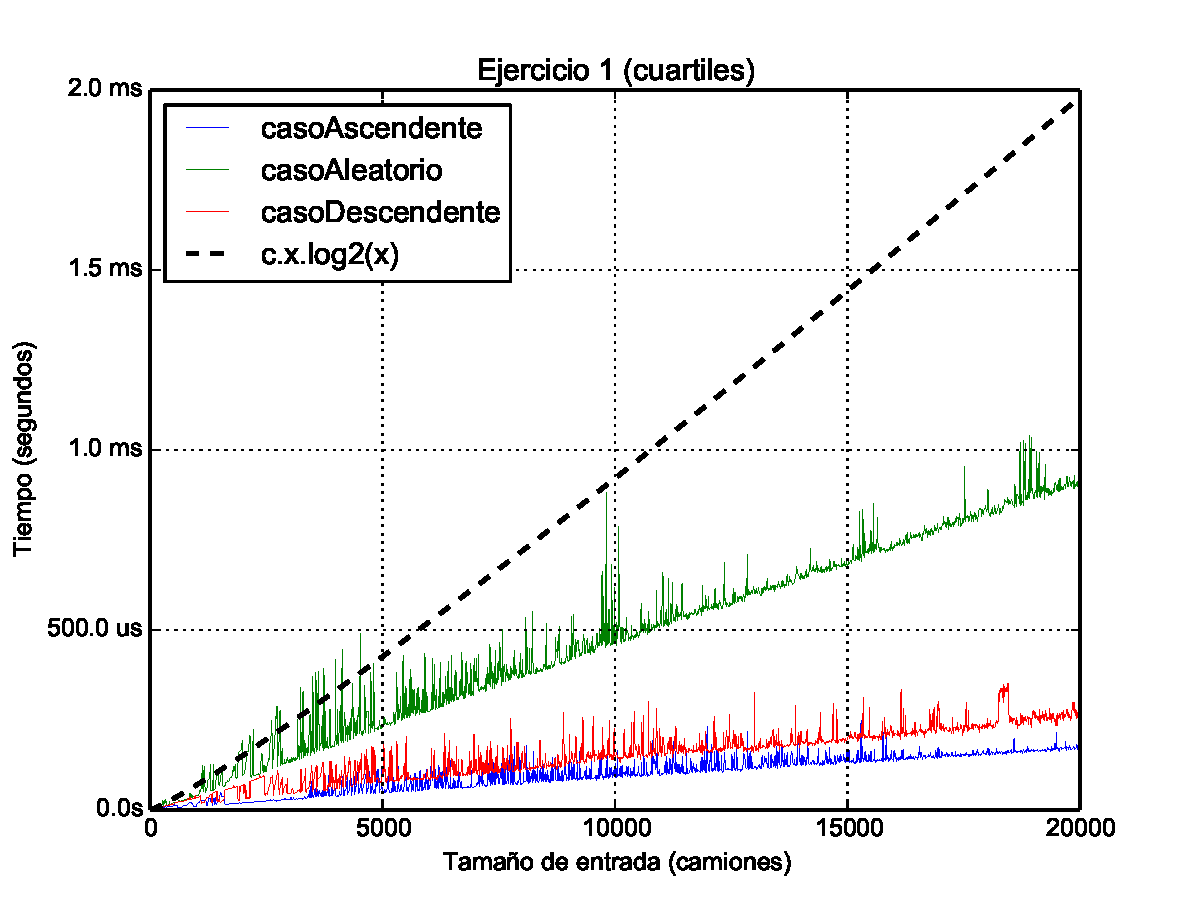
\includegraphics[width=1.4\textwidth,angle=90]{../ej1/graficos/test_1.pdf}
   \caption{\textbf{Muestreo general del Ejercicio 1}}
   \label{fig:ej1-1}
   \end{center}
\end{figure}

\clearpage
\begin{figure}[H]
   \begin{center}
   %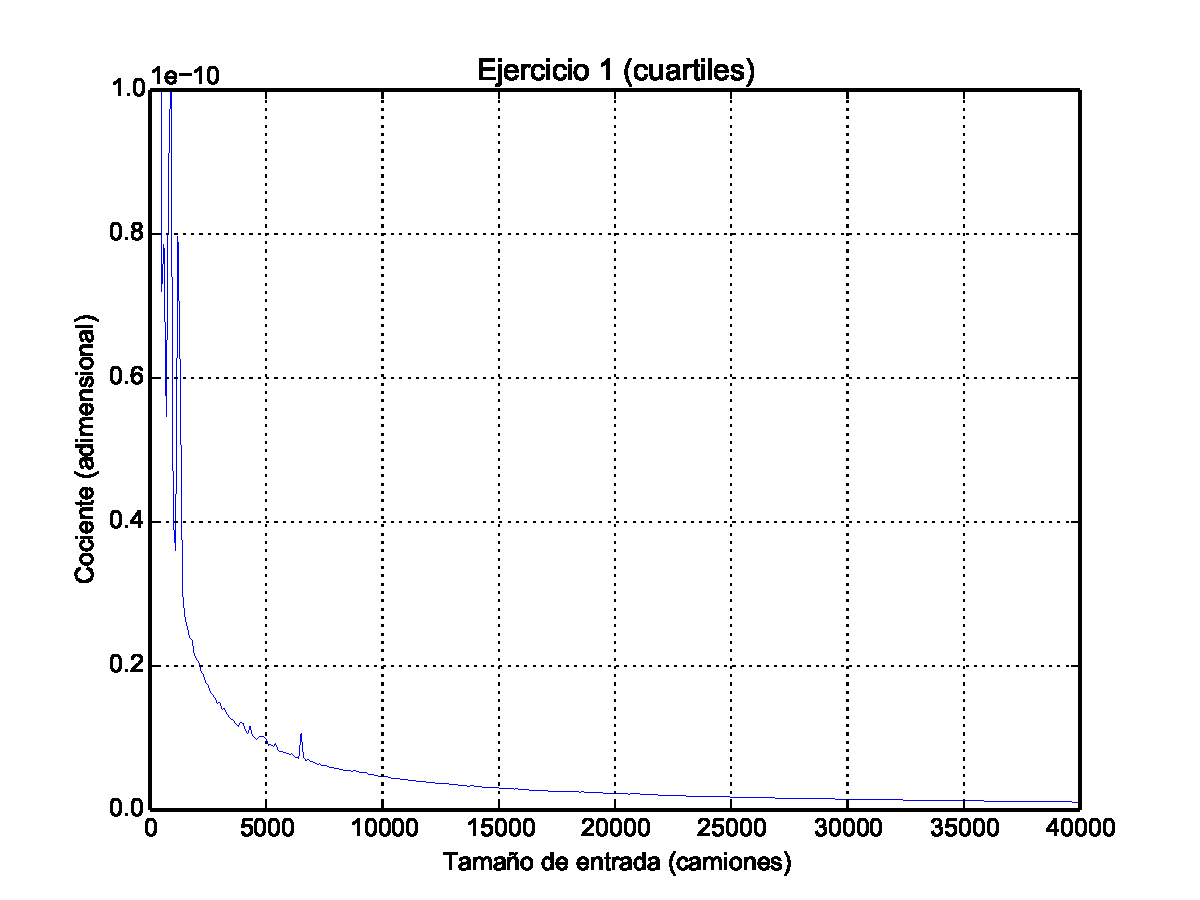
\includegraphics[width=1.4\textwidth,angle=90]{../ej1/graficos/test_2.pdf}
   \caption{\textbf{Relación contra $n^{2}$}}
   \label{fig:ej1-2}
   \end{center}
\end{figure}


Si bien como se explicó previamente y se plasmó en las figuras \ref{fig:ej1-1} y \ref{fig:ej1-2}
la complejidad del algoritmo está dada por el ordenamiento. Sin embargo también resulta interesante
analizar  otro factor que entra en juego en el rendimiento del algoritmo. La segunda parte
del algoritmo tiene un mejor caso en el cual la diferencia entre los entre la mayor fecha y la menor fecha
es menor o igual a \textit{intervaloInspector}. Si eso ocurre la condición de la guarda interna se cumple
en una primera iteración y la constante del ciclo se ve completamente amortizada. Sigue siendo lineal, pero
la constante resulta muy baja. El peor caso sería el caso contrario: Cada fecha está a mas de \textit{intervaloInspector}
días de su vecina. Esto significaría que para iteración del bucle exterior el iterador del final del intervalo 
solo puede avanzar un día, por lo tanto para cada elemento hay que realizar toda la lógica de comparación y descarte.

Esto significa que esa segunda parte, la parte lineal, funciona muy bien cuando hay mucha densidad de datos y pierde
eficacia cuando hay mucha dispersión de datos. Para contrastar esto lo que se hizo fue fijar un tamaño de entrada
(5000 camiones) y un intervalo de inspector ( 200 ) y generar diferentes casos de prueba, en los cuales lo que cambia
es la dispersión de los datos. Para eso lo que se hizo fue tomar intervalos de tamaño creciente y ubicar
todos los datos de entrada en esos intervalos ditribuidos uniformemente. Al aumentar el tamaño del intervalo
y distribuir los mismos datos en el intervalo lo que se obtiene es una menor densidad de datos. El intervalo
se midió en manera porcentual con respecto a \textit{intervaloInspector}. En la figura \ref{fig:ej1-3} se puede
apreciar este experimento.

Es interesante además notar que mientras el tamaño del intervalo no llega al 100\% de \textit{intervaloInspector}
el tiempo de mantiene completamente constante. Luego aumenta de manera claramente lineal. Por otra parte se puede
observar como la parte de ordenamiento se estabiliza rapidamente mientras que el tiempo total de ejecución aumenta debido
a la parte lineal del algorítmo.



\clearpage
\begin{figure}[H]
   \begin{center}
   %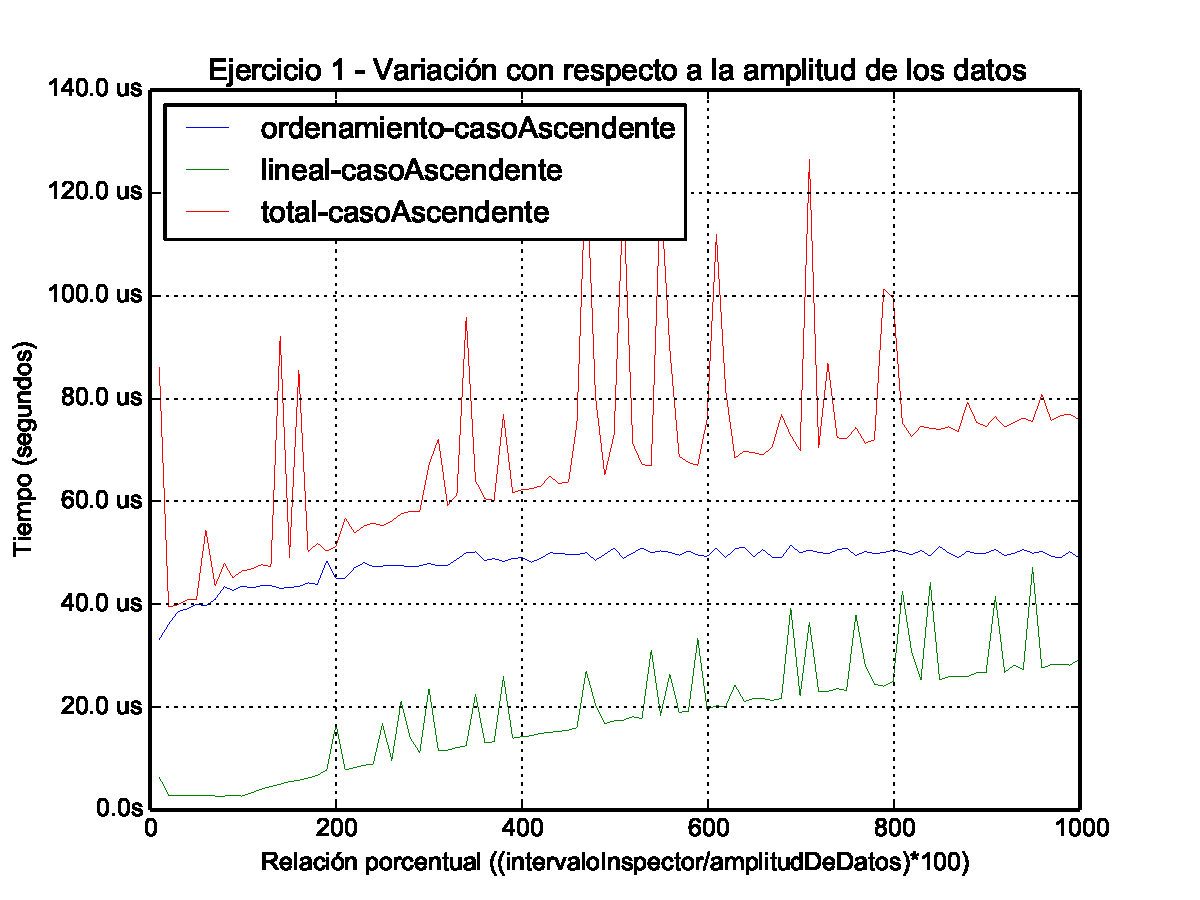
\includegraphics[width=1.4\textwidth,angle=90]{../ej1/graficos/test_3.pdf}
   \caption{Tiempo de ejecución contra dispersión de los datos}
   \label{fig:ej1-3}
   \end{center}
\end{figure}

%Gráfico1

%Lo siguiente lo dejo escrito pero hay que ver si hay tiempo para hacer todos esos tests... 

%Además, para comprobar que efectivamente la complejidad final está dominada por el algoritmo de sort, se compararon
%los tiempos de la primer parte del algoritmo ($Sort$) y la segunda ($Ciclos$). \\
%Se observa en el siguiente gráfico de $tiempo$ vs $n$:cantidad de camiones, que para el caso del $Sort$ los tiempos
%son mayores, pero siempre por debajo de la complejidad calculada.   

% Gráfico2

%Por último, se compararon los diferentes tiempos según se variaba la longitud $L$ del intervalo formado por 
%la mínima fecha y la máxima fecha en que pasan los camiones, dejando el parámetro $D$ período de contratación del 
%inspector fijo. \\
%Se puede observar que si $D$ es mayor a $L$ el tiempo aumenta como esperábamos, ya que se producen más iteraciones.

% Gráfico3 

% -----------------------------------------------
\end{document}
